\documentclass{article}

\begin{document}
    \marginnote{\textbf{\textit{VL 8}}\\24.04.2023, 11:45}

    \begin{Experiment}{Ladungsnachweis \href{https://de.wikipedia.org/wiki/Wimshurstmaschine}{Wimshurstmaschine} und \href{https://de.wikipedia.org/wiki/Fotoplatte}{Photoplatte}}
        Bestrahlen der Photoplatte mit und ohne Glasscheibe. Ohne Scheibe ist Ladungsabfall erkennbar, mit Scheibe nicht. Wir beobachten:
        \begin{itemize}
            \item Entladung einer negativ geladenen Zn-Photoplatte durch Bestrahlung mit Licht.
            \item Bei positiv geladener Platte verändert sich der Zeigerausschlag nicht. 
            \item Mit Glasplatte findet keine Entladung statt: der UV-Anteil des Lichtes wird von der Scheibe absorbiert.
        \end{itemize}
        Die quantitative Durchführung mit der \href{https://www.leifiphysik.de/quantenphysik/quantenobjekt-photon/versuche/h-bestimmung-mit-der-gegenfeldmethode}{Gegenfeldmethode} liefert folgende Beobachtungen:
        \begin{itemize}
            \item Beuleuchtung einer Metallplatte führt zur Induktion elektrischen Stroms und eines Auslösens von Elektronen ab einer gewissen Grenzfrequenz $f_\textit{gr}\in\R_{>0}$. 
            \item $\nu_\textit{gr}$ hängt von dem Material der Platte ab.
            \item $I$ hängt von der Intensität $P$ des Lichtes ab, $\nu_\textit{gr}$ jedoch nicht. 
            \item Ab einer negativen Spannung $U_\textit{max}$ wird der Stromfluss verhindert.
            \item $U_\textit{max}$ ist \emph{nicht} von $P$ abhängig. 
            \item $U_\textit{max}$ ist \emph{linear} von $\nu$ abhängig.
            \item Der Sättigungsstrom $I_S$ hängt \emph{liner} von $P$ ab.
            \item Die Elektronen werden verzögerungsfrei herausgelöst. 
        \end{itemize}
        Trägt man die Messdaten in Graphen auf, erhält man folgende Schemata:
        \begin{figure}[H]
            \centering
            \begin{subfigure}[b]{0.4\textwidth}
                \centering
                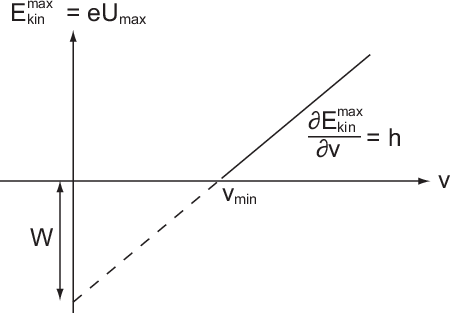
\includegraphics[width=5cm]{Bilddateien/UvonNu-Photoeffekt.png}
                \caption{$e\cdot U(\nu)$ aus \cite{ethz:Photoeffekt}.}
            \end{subfigure}
            \hspace{1cm}
            \begin{subfigure}[b]{0.4\textwidth}
                \centering
                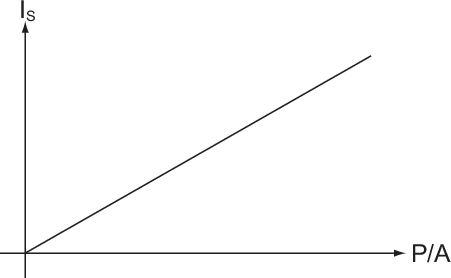
\includegraphics[width=5cm]{Bilddateien/Saettigungsstrom-Photoeffekt.png}
                \caption[short]{$I_S(P/A)$ aus \cite{ethz:Photoeffekt}.}
            \end{subfigure}
        \end{figure}
    \end{Experiment}

    Die Interpretation der experimentellen Befunde liefert Einstein: er stellt die \href{https://de.wikipedia.org/wiki/Quantenhypothese}{\emph{Lichtquantenhypothese}} auf. Sie postuliert folgende Annahmen:
    \begin{enumerate}
        \item Die einfallende Strahlung besteht aus \emph{Lichtquanten} (Photonen) mit Energie $E=h\cdot\nu$.
        \item Jedes absorbierte Photon gibt seine Energie vollständig an ein sogenanntes \emph{Photoelektron} (herausgelöstes Elektron) ab.
        \item Die Austrittsarbeit $W$ muss aufgebracht werden, um Elektronen aus dem Festkörper hinauslösen zu können: $h\cdot\nu > W_A$
        \item Für die kinetische Energie der Elektronen folgt $E_\textit{kin}^\textit{max}(\nu) = h\cdot\nu-W_A$. Haben die Atome die Anregungsenergie $E_B$, so muss zusätzlich noch berücksichtigt werden $E_\textit{kin}(\nu) = h\cdot\nu-W_A-E_B$. [$\to$ Niveausprung]
        \item Bei Gegenspannung $U=U_\textit{max}$ ist die Geschwindigkeit der Elektronen gleich Null: es gilt der Zusammenhang
        \[\frac{1}{2}\cdot m_e\cdot v_e^2 = e\cdot U_\textit{max} \stackrel{\textit{def }E_\textit{kin}^\textit{max}(\nu)}{\Longleftrightarrow} e\cdot\abs{U_{max}} = h\cdot\nu - W_A.\]
        Mit der Photonenenergie- und Impuls
        \[E_\textit{\gamma}(\nu) = h\cdot\nu =: \hbar\cdot \omega(\nu)\quad\&\quad p=\hbar\cdot k,\quad \hbar:=\frac{h}{2\cdot\pi}\]
        mit Wellenvektor $k\in\R^3$ und $p\in C^1(\R,\R^3)$ als Impuls, dann gilt mit \emph{Relativitätstheorie} gerade
        \[E^2 = p^2\cdot c_0^2 + m_0^2\cdot c_0^4 \stackrel{m_\gamma = 0}{\Longrightarrow} \dabs{p}{2} = \frac{E}{c_0} = \frac{\hbar\cdot\omega(\nu)}{c_0} \stackrel{(D)}{=} \hbar\cdot\dabs{k}{2},\]
        wobei bei $(D)$ die \emph{Dispersionsrelation} [$\to$ IK3-E] verwendet wurde.
    \end{enumerate}

    \begin{Aufgabe}
        \nr{} Rechne noch einmal die Dispersionsrelation nach. Wie lautet das Argumentationsergebnis für ein Elektron $e$ der Masse $m_e$?
    \end{Aufgabe}

    \subsubsection*{Der Compton Effekt}
        Der \href{https://de.wikipedia.org/wiki/Compton-Effekt}{\emph{Compton Effekt}} diente dem Nachweis des Teilchencharakters von Photonen, wobei wiefolgt der Versuch aufgebaut wurde:
        \begin{figure}[H]
            \centering
            \begin{subfigure}[b]{0.3\textwidth}
                \centering
                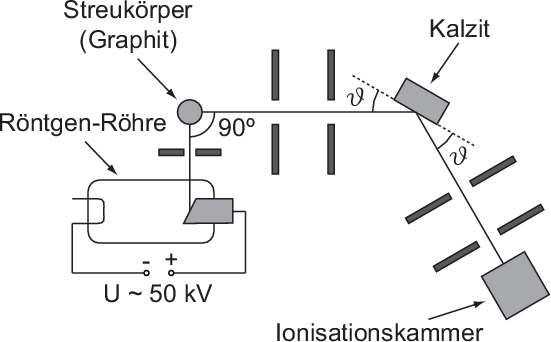
\includegraphics[width=4cm]{Bilddateien/ComptonAufbau.png}
                \caption{Versuchsaufbau.}
            \end{subfigure}
            \hspace{1cm}
            \begin{subfigure}[b]{0.3\textwidth}
                \centering
                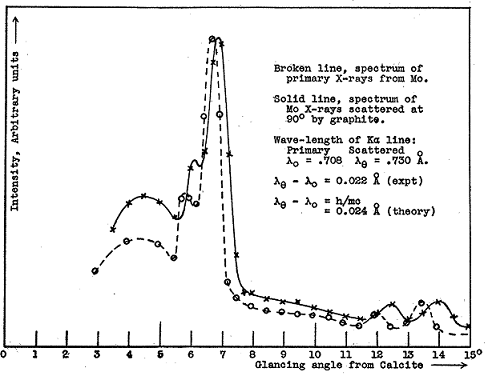
\includegraphics[width=4cm]{Bilddateien/ComptonEffektMessung.png}
                \caption{Messung.}
            \end{subfigure}
            \hspace{1cm}
            \begin{subfigure}[b]{0.3\textwidth}
                \centering
                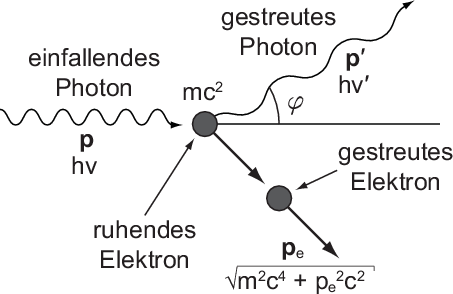
\includegraphics[width=4cm]{Bilddateien/ComptonKollision.png}
                \caption{Kollision.}
                \label{subfig:ComptonKollision}
            \end{subfigure}
            \caption{Compton Effekt aus \cite{ethz:ImpulsPhoton}.}
        \end{figure}
        Es zeigt dabei Abbildung \ref{subfig:ComptonKollision} die \emph{angenommene inelastische Kollision} eines Photons mit einem Elektron. Somit gelingt \emph{hier} der Brückenschlag aus der Quantenmechanik zur klassischen Mechanik des Zweierstoßes. Wir folgern mit Energieerhaltung
        \[\hbar\cdot\omega(\nu) + m_ec_0^2 = \hbar\cdot\omega(\tilde\nu) + E_e,\]
        wobei die $\hbar$ Terme das Photon und $E_e$ das Elektron beschreiben. Mit Impulserhaltung folgt
        \[p + 0_\Abb{\R}{\R^3} = \tilde p + p_e,\]
        sodaß $(1)^2 - (2)^2\cdot c_0^2$ den Zusammenhang
        \[\nsqbra{\hbar\cdot(\omega(\nu)-\omega(\tilde\nu)) + m_o\cdot c_0^2}^2 - (p-\tilde p)^2\cdot c_0^2 = E_e^2 - p_e^2\cdot c_0^2\]
        liefert, wobei unter $E=m_02c^4+c_0^2p^2$ ($p^2 = \scpr{p}{p}_{\R^3}$) folgt
        \[-2\cdot\hbar^2\cdot\omega(\nu)\cdot\omega(\tilde\nu) + 2\cdot\hbar\cdot(\omega(\nu)-\omega(\tilde\nu))\cdot m_0c_0^2 + 2\hbar^2\cdot\omega(\nu)\cdot\omega(\tilde\nu)\cdot\cos(\phi(\nu)) = 0\]
        für $\abs{\phi} = (\hbar\cdot\omega(\nu))/c_0$ und schlielich  
        \[\omega(\tilde\nu) = \frac{\omega(\nu)}{\hbar\omega(\nu)/(m_0\cdot c_0^2)\cdot (1-\cos(\phi(\nu))) + 1}.\]
        Für die Wellenlänge $\lambda_e(\nu) = 2\pi\cdot e/\omega(\nu)$ gilt letztlich 
        \[\Delta\lambda_e(\nu) = \frac{2\pi\cdot e}{\omega(\nu)\cdot\omega(\tilde\nu)}\cdot(\omega(\nu)-\omega(\tilde\nu)) =: \lambda_C\cdot (1-\cos(\phi(\nu))),\]
        wobei wir $\lambda_C:=h/(m_0\cdot c_0)\approx 2.4\cdot 10^{-12}\si\metre = 0.024\si\angstrom$ als \emph{Compton-Wellenlänge} definieren und die Gleichung $\lambda_e(\nu)$ als \emph{Compton-Streuung} bezeichnen. 
        
        \begin{Aufgabe}
            \nr{} Rechne die Herleitung der Compton-Streuung nach. Notiere zunächst die Voraussetzungen und halte dich fortfahrend an die ersten skizzierten Schritte, wobei du sauber die Terme ausmultiplizierst und kürzt. Orientiere dich zusätzlich an [$\to$ Demtröder, S. 80].
        \end{Aufgabe}

        \subsubsection*{Eigenschafen des Photons}
            Wir listen wieder einige Eigenschafen des Photons auf:
            \begin{itemize}
                \item Die Photonendichte wird beschrieben als $n = N/V = U_\textit{em} / (h\cdot\nu) = \epsilon_0\cdot E^2 / (h\cdot\nu)$.
                \item Der Photonenstrom definiert als $\dv{t} n = I/(h\cdot\nu) = n\cdot c_0$.
                \item Der Gesamtimpuls als $p = n\cdot\hbar\cdot k$ mit Wellenvektor $k\in\R^3$ oder $\abs{\phi} = n\cdot h/\lambda = U_\textit{em} / c_0$. 
                \item Der Drehimpuls als $L = \pm \hbar\cdot k / \dabs{k}{2}$. 
            \end{itemize}
            Der Spin ist also Ganzzahlig, wodurch die Photonen den \emph{Bosonen} zugeordnet wird. 

        \subsubsection*{Welle-Teilchen-Dualismus}
            Der \href{https://de.wikipedia.org/wiki/Welle-Teilchen-Dualismus}{\emph{Welle-Teilchen-Dualismus}} ist ein zentrales Konzept der Quantenmechanik, welches besagt, daß jedes Teilchen sowohl Wellen- als auch Teilcheneigenschaften besitzt. Dieses Konzept wurde von \href{https://de.wikipedia.org/wiki/Louis_de_Broglie}{\emph{Louis de Broglie}} eingeführt. Er verknüpfte den Impuls $p\in\R^3$ mit dem Wellenvektor $k\in\R^3$ durch $p = \hbar\cdot k$ und der \href{https://de.wikipedia.org/wiki/Materiewelle}{\emph{de Broglie Wellenlänge}}. 
\end{document}